\chapter{Elementi orbitali}
\label{chap:elementi-orbitali}

Nel precedente capitolo abbiamo determinato l'equazione
dell'orbita~\eqref{eq:orbita} che lega la coordinata polare $r$ all'anomalia
vera $\chi$, che dipende a sua volta dal tempo. La seconda legge di Keplero,
però, ci dice che $\chi$ non varia in maniera costante con il tempo, eccetto nel
caso particolare di orbita circolare. In questo capitolo ci occuperemo della
determinazione della posizione, in un dato istante di tempo, della particella
relativa che si muove su un'orbita ellittica.

\section{Equazione di Keplero}
\label{sec:equazione-keplero}

\begin{figure}
  \centering
  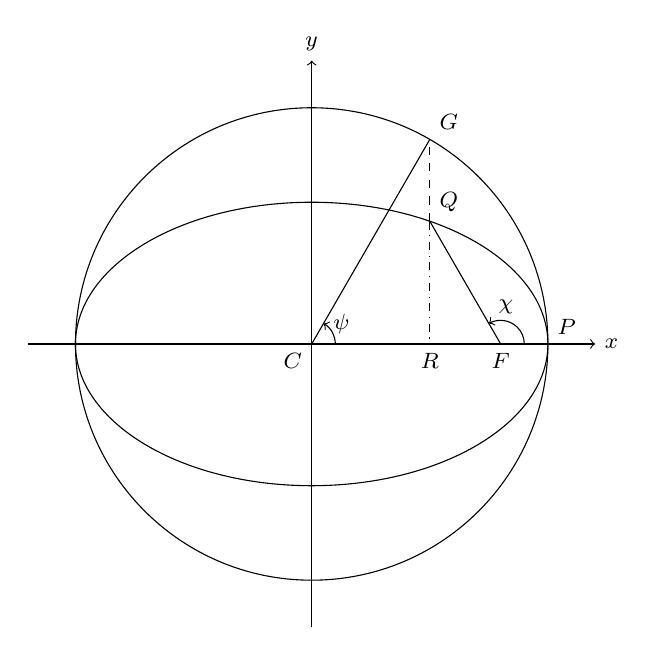
\begin{tikzpicture}[font=\footnotesize,scale=3]
    % a=1, e=0.8, b=a*sqrt(1-e^2)=0.6, c=ae=0.8, p=a*(1-e^2)=0.36, chi=120,
    % r(chi)=0.6, x_Q=x_G=c+r(chi)*cos(chi)=0.5,
    % y_Q=r(chi)*sin(chi)=0.5196, y_G=y_Q*a/b=0.866, psi=60 (deriva dalla relazione
    % fra anomalia vera ed eccentrica)
    \draw [->] (-1.2,0) -- (1.2,0) node[right] {$x$}; %asse x
    \draw [->] (0,-1.2) -- (0,1.2) node[above] {$y$}; %asse y
    \draw (0,0) circle (1); % circonferenza ausiliaria
    \draw (0,0) ellipse (1 and 0.6); %ellisse
    \draw (0.8,0) -- (0.5,0.5196) node[above right] {$Q$}; % segmento FQ
    \draw [dashed] (0.5,0.5196) -- (0.5,0.866); % segmento QG
    \draw (0,0) -- (0.5,0.866) node[above right] {$G$}; % segmento CG
    \draw (0,0) node[below left] {$C$}; % etichetta del punto C
    \draw (0.8,0) node[below] {$F$}; % etichetta del punto F
    \draw (1,0) node[above right] {$P$}; % etichetta del punto P
    \draw [dashdotted] (0.5,0.5196) -- (0.5,0) node[below] {$R$}; % segmento RQ
    \draw [->] (0.9,0) arc (0:120:0.1) node[above right] {$\chi$}; % angolo chi
    \draw [->] (0.1,0) arc (0:60:0.1) node[right] {$\psi$}; % angolo psi
  \end{tikzpicture}
  \caption[Ellisse e circonferenza ausiliaria per l'equazione di
  Keplero]{Ellisse e circonferenza ausiliaria concentrica. Abbiamo posto $a=1$
    ed $e=0.8$}
  \label{fig:circonferenza-ausiliaria-keplero}
\end{figure}
La seconda legge di Keplero permette di trovare la posizione relativa di un
corpo di un sistema binario in un qualsiasi istante di tempo. Con riferimento
alla figura~\ref{fig:circonferenza-ausiliaria-keplero}, il punto $Q$
dell'ellisse indica la posizione del corpo all'istante di tempo $t$ e $P$ la
posizione del periapside, da cui il corpo passa all'istante
$t_0$. Nell'intervallo di tempo $\mathopen{[}t_0, t\mathclose{]}$ il raggio
vettore che congiunge il fuoco $F$ alla posizione del corpo sull'ellisse si
sposta da $FP$ a $FQ$, spazzando dunque l'area $FPQ$. Allora per la seconda
legge di Keplero
\begin{equation}
  \text{area } FPQ : \text{area ellisse} = t-t_0 : T,
\end{equation}
da cui otteniamo
\begin{equation}
  \text{area } FPQ = \frac{\pi ab(t-t_0)}{T}.
\end{equation}
Definendo la \emph{velocità angolare media} $\omega = 2\pi/T$ questa equazione
diventa
\begin{equation}
  \text{area } FPQ = \frac{1}{2}\omega ab(t-t_0).
\end{equation}
Conoscendo l'istante di passaggio al periapside $t_0$, il periodo di rivoluzione
$T$, il semiasse maggiore $a$ e l'eccentricità $e$, legata al semiasse minore
dalla~\eqref{eq:semiasse-minore-ellisse}, è possibile calcolare in un qualsiasi
istante di tempo $t$ l'area $FPQ$ da cui si ricava la posizione $Q$. Sebbene
questa tecnica sia molto semplice teoricamente, è poco utile nella pratica. Si
usa invece il metodo che ci apprestiamo a illustrare.

Circoscriviamo all'ellisse una circonferenza ausiliaria di raggio $a$ e
concentrica con l'ellisse, come nella
figura~\ref{fig:circonferenza-ausiliaria-keplero}.  Sia $G$ l'intersezione con
la circonferenza della perpendicolare all'asse $x$ innalzata dal punto $Q$. Se
$\chi > \pi$, il punto $G$ apparterrà alla semicirconferenza inferiore. L'angolo
$G\widehat{C}P$, dove $C$ è il centro della circonferenza, è chiamato
\emph{anomalia eccentrica} e lo indicheremo con $\psi$. L'anomalia eccentrica
può assumere valori fra $0$ e $2\pi$ e al periapside si ha $\psi = \chi = 0$,
all'apoapside $\psi = \chi = \pi$. I punti $Q=(x_Q,y_Q)$ e $G=(x_Q,y_G)$ hanno
la stessa ascissa e vogliamo trovare una relazione fra le loro ordinate. Per
fare questo ricordiamo che l'equazione cartesiana di una circonferenza di raggio
$a$ e centro l'origine del sistema di riferimento $x_\textup{c}Oy_\textup{c}$ è
\begin{equation}
  x_\textup{c}^2 + y_\textup{c}^2 = a^2.
\end{equation}
Invece, l'equazione di un'ellisse con centro nell'origine del sistema
$x_\textup{e}O'y_\textup{e}$ e semiassi maggiore $a$, lungo l'asse
$x_\textup{e}$, e minore $b$, lungo l'asse $y_\textup{e}$, è
\begin{equation}
    \frac{x_\textup{e}^2}{a^2} + \frac{y_\textup{e}^2}{b^2} = 1.
\end{equation}
Se gli assi dei sistemi di riferimento delle due coniche sono coincidenti, come
nel nostro caso, uguagliando le ascisse risulta
\begin{equation}
  x_\textup{c}^2 = x_\textup{e}^2 \iff a^2 - y_\textup{c}^2 = a^2 -
  y_\textup{e}^2a^2/b^2 \iff \abs{y_\textup{c}} = \abs{y_\textup{e}}a/b.
\end{equation}
Allora, per i punti $Q$ e $G$ abbiamo che $y_G = y_Qa/b$, poiché $y_G$ e $y_Q$
hanno sempre lo stesso segno. D'altra parte, $y_Q = r\sin\chi$ e
$y_G = a\sin\psi$, cioè
\begin{equation}
  \label{eq:r-sin-chi}
  r\sin\chi = b\sin\psi.
\end{equation}
Inoltre $\overline{FR} =
r\cos\chi$,\footnote{Un
  valore negativo di $\overline{FR}$ indica che il punto $R$ si trova alla
  sinistra di $F$ sull'asse $x$.} ma è anche $\overline{FR} = \overline{CR} -
\overline{CF} = a\cos\psi - ae$, da cui
\begin{equation}
  \label{eq:r-cos-chi}
  r\cos\chi = a(\cos\psi - e).
\end{equation}
Sommando membro a membro i quadrati delle equazioni~\eqref{eq:r-sin-chi}
e~\eqref{eq:r-cos-chi} otteniamo
\begin{equation}
  \begin{split}
    r^2 &= r^2\cos^2\chi + r^2\sin^2\chi = a^2(\cos\psi - e)^2 + b^2\sin^2\psi\\
    &= a^2\cos^2\psi-2a^2e\cos\psi+a^2e^2+a^2\sin^2\psi-a^2e^2\sin^2\psi\\
    &= a^2(1+e^2-2e\cos\psi-e^2\sin^2\psi) = a^2(1-2e\cos\psi+e^2\cos^2\psi)\\
    &= a^2(1 - e\cos\psi)^2,
  \end{split}
\end{equation}
da cui ricaviamo la seguente equazione che lega la coordinata polare $r$ con
l'anomalia eccentrica $\psi$
\begin{equation}
  \label{eq:r-anomalia-eccentrica}
  r = a(1 - e\cos\psi).
\end{equation}
Dall'equazione~\eqref{eq:terza-legge-keplero} che esprime la terza legge di
Keplero
\begin{equation}
  \omega^2 = \frac{4\pi^2}{T^2} = \frac{GM_\textup{T}}{a^3}.
\end{equation}
Ricordando la~\eqref{eq:reciproco-semilato}, la~\eqref{eq:semilato-ellisse} e
la~\eqref{eq:velocita-tangenziale} abbiamo
\begin{equation}
  \begin{split}
    r^2\dot{\chi}^2 &= \frac{l_0^2}{\mu^2p^2}(1 + e\cos\chi)^2 =
    \frac{l_0^2}{\mu^2p} \frac{(1+e\cos\chi)^2}{a(1-e^2)} \\
    &= GM_\textup{T} \frac{(1+e\cos\chi)^2}{a(1-e^2)} = \omega^2a^3
    \frac{(1+e\cos\chi)^2}{a(1-e^2)} \\
    &= \omega^2a^4 \frac{(1+e\cos\chi)^2}{a^2(1-e^2)^2}(1-e^2) =
    \frac{\omega^2a^4(1-e^2)}{r^2}.
  \end{split}
\end{equation}
Quindi, dalla~\eqref{eq:velocita-ellisse}, il quadrato della derivata temporale
di $r$ è
\begin{equation}
  \begin{split}
    \dot{r}^2 &= v^2 - r^2\dot{\chi}^2 = GM_\textup{T}
    \left(
      \frac{2}{r} - \frac{1}{a}
    \right) - \frac{\omega^2a^4(1-e^2)}{r^2} \\
        &= \omega^2a^3
    \left(
      \frac{2}{r} - \frac{1}{a}
    \right) - \frac{\omega^2a^4(1-e^2)}{r^2} \\
    &= \frac{2\omega^2a^3r-r^2\omega^2a^2-\omega^2a^4+\omega^2a^4e^2}{r^2}\\
    &= \frac{\omega^2a^2}{r^2}(a^2e^2-(r-a)^2)
  \end{split}
\end{equation}
da cui
\begin{equation}
  \toder{r}{t} = \dot{r} = \frac{\omega a}{r}\sqrt{a^2e^2 - (r-a)^2}.
\end{equation}
Per risolvere questa equazione differenziale ordinaria cambiamo la funzione
incognita da $r$ in $\psi$ effettuando la
sostituzione~\eqref{eq:r-anomalia-eccentrica}. Deriviamo
la~\eqref{eq:r-anomalia-eccentrica} rispetto al tempo
\begin{equation}
  \dot{r} = ae\dot{\psi}\sin\psi.
\end{equation}
Sostituiamo la~\eqref{eq:r-anomalia-eccentrica} nell'equazione differenziale
\begin{equation}
  r = \frac{\omega a\sqrt{a^2e^2 - a^2e^2\cos^2\psi}}{a(1-e\cos\psi)} =
  \frac{\omega ae\sin\psi}{1-e\cos\psi}.
\end{equation}
Uguagliando le due espressioni di $\dot{r}$ così ottenute ricaviamo
\begin{equation}
  \toder{\psi}{t} = \dot{\psi} = \frac{\omega}{1-e\cos\psi}.
\end{equation}
Ricordando che al perielio abbiamo $t = t_0$ e $\psi = 0$, integriamo questa
equazione differenziale fino a un generico istante di tempo $t$ in cui
l'anomalia eccentrica vale $\psi$
\begin{gather}
  \int_{t_0}^t \omega\dd \tau = \int_0^\psi(1-e\cos\psi')\dd \psi' \iff\\
  \phi = \omega(t - t_0) = \psi - e\sin\psi, \label{eq:keplero}
\end{gather}
dove $\phi = \omega(t-t_0)$ è chiamata \emph{anomalia media}. Anche l'anomalia
media varia fra $0$, valore raggiunto per $t = t_0$ cioè al periapside, e
$2\pi$. Il corpo relativo passa all'apoapside all'istante $t = t_0 + T/2$,
quindi in questo punto $\phi = \psi = \chi = \pi$. La~\eqref{eq:keplero} è detta
\emph{equazione di Keplero}. In ogni fissato istante di tempo $t$, la sua
soluzione $\psi$ permette di ricavare, tramite
la~\eqref{eq:r-anomalia-eccentrica}, la coordinata polare $r$. Inoltre possiamo
determinare una relazione tra l'anomalia eccentrica e l'altra coordinata polare
$\chi$. Infatti, uguagliando i secondi membri delle equazioni~\eqref{eq:orbita}
e~\eqref{eq:r-anomalia-eccentrica} abbiamo
\begin{equation}
  \begin{aligned}
    a(1-e\cos\psi) &= \frac{a(1-e^2)}{1+e\cos\chi} \iff 1+e\cos\chi =
    \frac{1-e^2}{1-e\cos\psi} \iff \\
    e\cos\psi &= \frac{1-e^2-1+e\cos\psi}{1-e\cos\psi} =
    \frac{e(\cos\psi-e)}{1-e\cos\psi} \iff \\
    \cos\psi &= \frac{\cos\psi-e}{1-e\cos\psi}.
  \end{aligned}
\end{equation}
Aggiungiamo e sottraiamo ambo i membri dell'ultima equazione da $1$
\begin{align}
  \begin{split}
    1-\cos\chi &= 1-\frac{\cos\psi-e}{1-e\cos\psi} =
    \frac{1-e\cos\psi-\cos\psi+e}{1-e\cos\psi} \\
    &= \frac{(1+e)(1-\cos\psi)}{1-e\cos\psi},
  \end{split} \\
  \begin{split}
    1+\cos\chi &= 1+\frac{\cos\psi-e}{1-e\cos\psi} =
    \frac{1-e\cos\psi+\cos\psi-e}{1-e\cos\psi} \\
    &= \frac{(1-e)(1+\cos\psi)}{1-e\cos\psi}.
  \end{split}
\end{align}
Facendo il rapporto dei primi e ultimi membri di queste equazioni troviamo
la relazione cercata
\begin{gather}
  \frac{1-\cos\chi}{1+\cos\chi} = \frac{1+e}{1-e}\frac{1-\cos\psi}{1+\cos\psi}
  \iff \\
  \tan^2\frac{\chi}{2} = \frac{1+e}{1-e}\tan^2\frac{\psi}{2}.
\end{gather}
In questa equazione possiamo esplicitare $\chi$ in funzione di $\psi$
\begin{equation}
  \chi = 2\arctan
  \left(
    \sqrt{\frac{1+e}{1-e}}\tan\frac{\psi}{2}
  \right).
\end{equation}
Il risultato è corretto, però con questa definizione di $\chi$ c'è una
discontinuità di prima specie in $\psi = \pi$ perché la tangente è discontinua
in $\pi/2$. Per rendere continua $\chi$ in funzione di $\psi$ dobbiamo
aggiungere $\pi$ al valore dell'arcotangente se $\psi > \pi$, cioè
\begin{equation}
  \label{eq:anoamlie-vera-eccentrica}
  \chi =
  \begin{cases}
    2\arctan
  \left(
    \sqrt{\dfrac{1+e}{1-e}}\tan\dfrac{\psi}{2}
  \right) & \text{se $0 \leq \psi \leq \pi$,}
    \\[2.0ex]
  2
  \left(
    \arctan
    \left(
      \sqrt{\dfrac{1+e}{1-e}}\tan\dfrac{\psi}{2}
    \right) + \pi
  \right) & \text{se $\pi < \psi \leq 2\pi$.}
  \end{cases}
\end{equation}

\section{Soluzioni dell'equazione di Keplero}
\label{sec:soluzioni}

L'equazione di Keplero~\eqref{eq:keplero} è trascendente nell'incognita $\psi$
per via del termine $\sin\psi$, e non ammette una soluzione elementare, ma
possono essere utilizzati diversi metodi numerici per risolverla.

\subsection{Metodo di Newton~-~Raphson}
\label{sec:newton}

Il primo metodo che utilizzeremo per determinare il valore dell'anomalia
eccentrica $\psi$ in corrispondenza di un fissato istante di tempo $t$ è quello
di Newton~-~Raphson (\textcite[30]{brugnano:calcolo-numerico}), chiamato anche
\emph{metodo delle tangenti}, descritto nel seguente
\begin{teorema}[di Newton~-~Raphson]
  Sia $f\in C^2(\mathopen{[}a,b\mathclose{]})$, con
  $\mathopen{[}a,b\mathclose{]}\subset\R$. Se
  \begin{subequations}
    \begin{gather}
      f(a)f(b) <0, \label{eq:esistenza-zero}\\
      f'(x) \neq 0 \quad \forall x \in \mathopen{[}a,b\mathclose{]},\\
      f''(x) \neq 0 \quad \forall x \in \mathopen{[}a,b\mathclose{]},
    \end{gather}
  \end{subequations}
  allora, posto
  \begin{subequations}
    \begin{align}
      x_0 &=
      \begin{cases}
        a & \text{se $ f(a)f''(a)>0$,}\\
        b & \text{se $f(b)f''(b)>0$,}
      \end{cases}\\
      x_{n+1} &= x_n - \frac{f(x_n)}{f'(x_n)} \label{eq:formula-newton}
    \end{align}
  \end{subequations}
  si ha che
  \begin{subequations}
    \begin{gather}
      \lim_n x_n = \tilde{x},\\
      f(\tilde{x}) = 0.
    \end{gather}
  \end{subequations}
\end{teorema}
Se la radice cercata ha molteplicità $1$ l'ordine di convergenza di questo
metodo è quadratico, altrimenti è lineare. Il teorema enunciato fornisce una
condizione sufficiente, ma non necessaria, per la convergenza della
successione~\eqref{eq:formula-newton} a una radice della funzione
$f$. Utilizzeremo il metodo iterativo descritto nel teorema senza preoccuparci
di verificare che tutte le ipotesi siano soddisfatte.

Fissate l'eccentricità $e$ e la velocità angolare media $\omega$, indichiamo con
$f(\psi) = \psi -e\sin\psi-\omega t$, $\psi\in\mathopen{[}0, 2\pi\mathclose{]}$,
la funzione di cui vogliamo trovare le radici $\psi$ in corrispondenza di un
istante di tempo $t$. Osserviamo che $f''(\psi) = e\sin\psi$, quindi
$f\in C^2(\R)$. Inoltre $f(0)f(2\pi) <
0$,\footnote{Si
  ha $f(0)f(2\pi) = 0$ solo se $\omega t = 0$ oppure $\omega t = 2\pi$, ma in
  questi casi si può verificare per sostituzione che la radice della funzione è
  $\psi = \omega t$, pertanto possiamo escluderli.}
quindi per il teorema di esistenza degli zeri, di cui la
condizione~\eqref{eq:esistenza-zero} è una delle ipotesi, all'interno
dell'intervallo $\mathopen{[}0, 2\pi\mathclose{]}$ esiste almeno una radice
della funzione $f$. Poiché
$f'(\psi) = 1 - e\cos\psi > 0 \quad \forall \psi\in\R$ e $f'$ è continua, la
radice è unica. Dall'equazione di Keplero abbiamo che $\psi$ differisce da
$\omega t$ per un termine dell'ordine di $e$, quindi poniamo come punto iniziale
$\psi_0 = \omega t$. Se $f(\psi_0)\neq 0$, cerchiamo un nuovo punto $\psi_1$ con
la formula~\eqref{eq:formula-newton} e valutiamo $f$ in $\psi_1$. Se è uguale a
$0$ allora abbiamo trovato la radice, altrimenti continuiamo nello stesso modo
finché non troviamo lo zero della funzione. Dopo aver determinato il valore di
$\psi$ al tempo $t$ possiamo anche ricavare la distanza $r$ dal fuoco con
la~\eqref{eq:r-anomalia-eccentrica} e l'anomalia vera $\chi$ con
la~\eqref{eq:anoamlie-vera-eccentrica}.

Ho scritto un programma con il linguaggio C che risolve l'equazione di Keplero
in più istanti del moto di rivoluzione della particella relativa e per diversi
valori dell'eccentricità dell'orbita. Il programma restituisce come output un
file contenente i valori dell'anomalia eccentrica, della distanza dal fuoco e
dell'anomalia vera in funzione del tempo per le differenti eccentricità fornite
come input. Il codice sorgente del programma è riportato
nell'appendice~\ref{cha:soluzione-keplero}. Nelle
figure~\ref{fig:newton-anomalia_eccentrica}, \ref{fig:newton-raggio}
e~\ref{fig:newton-anomalia_vera}, realizzate con il softawre \verb|gnuplot|,
sono rappresentati i risultati della simulazione. Per tutti i grafici, il
periodo di rivoluzione è $T = \SI{10}{\hour}$, l'istante di passaggio dal
periapside è $t_0 = 0$ e il semiasse maggiore vale $a =
\SI{2.5e6}{\kilo\metre}$,
quindi per la terza legge di Keplero
$GM_\textup{T} \simeq \SI{5e11}{\cubic\kilo\metre\per\square\second}$.
\begin{figure}
  \centering
  \input{keplero/newton-anomalia_eccentrica}
  \caption[Anomalia eccentrica in funzione del tempo con il metodo di
  Newton~-~Raphson]{Anomalia eccentrica in funzione del tempo calcolata
    utilizzando il metodo di Newton~-~Raphson}
  \label{fig:newton-anomalia_eccentrica}
\end{figure}
\begin{figure}
  \centering
  \input{keplero/newton-raggio}
  \caption[Distanza dal fuoco in funzione del tempo con il metodo di
  Newton~-~Raphson]{Distanza dal fuoco in funzione del tempo calcolata con
    la~\eqref{eq:r-anomalia-eccentrica} dopo aver trovato l'anomalia eccentrica
    con il metodo di Newton~-~Raphson}
  \label{fig:newton-raggio}
\end{figure}
\begin{figure}
  \centering
  \input{keplero/newton-anomalia_vera}
  \caption[Anomalia vera in funzione del tempo con il metodo di
  Newton~-~Raphson]{Anomalia vera in funzione del tempo calcolata con
    la~\eqref{eq:anoamlie-vera-eccentrica} dopo aver trovato l'anomalia
    eccentrica con il metodo di Newton~-~Raphson}
  \label{fig:newton-anomalia_vera}
\end{figure}

\subsection{Coefficienti di Bessel}
\label{sec:bessel}

Per risolvere l'equazione di Keplero utilizzeremo in questo paragrafo le
\emph{funzioni di Bessel di ordine intero}, o \emph{coefficienti di
  Bessel} (si vedano \textcites{abramowitz:handbook}{watson:bessel}%
{whittaker:modern-analysis}), che ora introdurremo.

La funzione $f(x,z)\colon\C\times\C\to\C$ definita da
\begin{equation}
  f(x,z) = \e^{(x/2)(z - 1/z)}
\end{equation}
è olomorfa in $\C\setminus 0$ rispetto alla variabile $z$, quindi può essere
espansa in serie di Laurent (\textcite[673]{demarco:analisi2}) di potenze di $z$
intorno a $z=0$
\begin{equation}
  f(x,z) = \sum_{n = -\infty}^{+\infty} c_n(x) z^n.
\end{equation}
Per il teorema di Laurent, i coefficienti $c_n(x)$, che indicheremo d'ora in poi
con $J_n(x)$, sono dati da
\begin{equation}
  J_n(x) = \frac{1}{2\pi\uimm}\int_\gamma \frac{\e^{(x/2)(z-1/z)}}{z^{n+1}}\dd z,
  \quad n\in\Z,
\end{equation}
in cui $\gamma$ è un qualsiasi circolo centrato nell'origine. Si dimostra che se
$n$ è un intero non negativo si ha (\textcite[355]{whittaker:modern-analysis})
\begin{equation}
  J_n (x) = \sum_{m = 0}^{+\infty}\frac{(-1)^m(x/2)^{n+2m}}{m!(n+m)!}.
\end{equation}
Per ottenere l'espressione di $J_n(x)$ con $n$ intero negativo osserviamo che
$f(x,z) = f(x,-1/z)$, quindi, espandendo in serie di Laurent,
\begin{equation}
  \begin{split}
    f(x,-1/z) &= \sum_{n = -\infty}^{+\infty}J_n(x)
    \left(
      -\frac{1}{z}
    \right)^n = \sum_{n = -\infty}^{+\infty}J_n(x)(-1)^nz^{-n} \\
    &= \sum_{n = -\infty}^{+\infty}J_{-n}(x)z^{-n}
  \end{split}
\end{equation}
da cui ricaviamo la formula
\begin{equation}
  J_{-n}(x) = (-1)^nJ_n(x).
\end{equation}
La funzione $J_n(x)$ è chiamata \emph{coefficiente di Bessel di argomento $x$ e
  ordine $n$}, mentre la funzione $f(x,z)$ è la \emph{funzione generatrice del
  coefficiente di Bessel}. Si dimostrano inoltre le seguenti formule ricorsive
(\textcites[17]{watson:bessel}[359]{whittaker:modern-analysis})
\begin{subequations}
  \begin{gather}
    \frac{2n}{x} J_n(x) = J_{n-1}(x) + J_{n+1}(x),\\
    J_n'(x) = \frac{J_{n-1}(x) - J_{n+1}(x)}{2} = \frac{n}{x}J_n(x) - J_{n+1} =
    J_{n-1} - \frac{n}{z}J_n,\\
    J_n''(x) = \frac{n^2}{x^2}J_n(x) - J_n(x) - \frac{1}{x}J_n'(x),\\
    \toder{}{x}(x^nJ_n(x)) = x^nJ_{n-1}(x),\\
    \toder{}{x}(x^{-n}J_n(x)) = -xJ_{n+1}(x).
  \end{gather}
\end{subequations}
Si può verificare, grazie alle relazioni appena riportate, che la funzione
$J_n(x)$ soddisfa la seguente equazione differenziale nell'incognita $y(x)$
\begin{equation}
  \toder[2]{y}{x} + \frac{1}{x}\toder{y}{x} +
  \left(
    1 - \frac{n^2}{x^2}
  \right)y = 0.
\end{equation}
Questa è l'\emph{equazione differenziale di Bessel per funzioni di ordine
  $n$}. Si può dare la seguente \emph{rappresentazione integrale dei
  coefficienti di Bessel}
(\textcites[20]{watson:bessel}[362]{whittaker:modern-analysis})
\begin{equation}
  \label{eq:bessel-integrale}
  J_n(x) = \frac{1}{\pi} \int_0^\pi\cos(n\theta - x\sin\theta)\dd\theta,
\end{equation}
quindi, derivando sotto il segno di integrale, abbiamo anche
\begin{equation}
  \label{eq:bessel-derivata-integrale}
  J_n'(x) = \frac{1}{\pi}\int_0^\pi\sin(n\theta - x\sin\theta)
  \sin\theta\dd\theta.
\end{equation}

Ritorniamo al problema fisico. Definiamo la funzione $G(\psi,\phi) = \psi -
e\sin\psi - \psi$, con $\psi,\phi\in\mathopen{[}0,
2\pi\mathclose{]}$. Dall'equazione di Keplero abbiamo $G(\psi(t),\phi(t)) = 0$
in ogni istante di tempo $t\in\mathopen{[}t_0,T+t_0\mathclose{]}$ e inoltre
$G_\psi(\psi(t),\phi(t)) = 1 - e\cos\psi(t) \neq 0$,
$\forall\psi\in\mathopen{[}0, 2\pi\mathclose{]}$ e $G\in C^1(\mathopen{[}0,
2\pi\mathclose{]}^2)$, quindi per il teorema del Dini
(\textcite[267]{demarco:analisi2}) esiste un'unica funzione di classe $C^1$ che
esplicita $\psi(t)$ rispetto a $\phi(t)$, per ogni
$t\in\mathopen{[}t_0,T+t_0\mathclose{]}$. Tuttavia, come già detto, non possiamo
dare un'espressione elementare della funzione $\psi(\phi)$, però possiamo
cercare un'espressione che coinvolga i coefficienti di Bessel, che sono funzioni
speciali. Notiamo innanzitutto che $\psi$ è una funzione dispari di
$\phi$. Finora ci siamo limitati a considerare gli intervalli
$\psi,\phi\in\mathopen{[}0, 2\pi\mathclose{]}$, però il moto della particella
relativa è periodico, quindi anche la funzione $\psi(\phi)$ è periodica, di
periodo $2\pi$.  La funzione $\ltoder{\psi(\phi)}{\phi}$ è integrabile
nell'intervallo $\mathopen{[}-\pi, \pi\mathclose{]}$ essendo continua, quindi è
sviluppabile in serie di Fourier (\textcite[440]{demarco:analisi2}) in media
quadratica in $\mathopen{[}-\pi, \pi\mathclose{]}$. Inoltre, poiché $\psi(\phi)$
è dispari, $\ltoder{\psi(\phi)}{\phi}$ è pari, quindi nello sviluppo
compariranno solo il termine costante e quelli in coseno, cioè
\begin{equation}
  \toder{\psi}{\phi} = \frac{a_0}{2} + \sum_{n=1}^{+\infty}a_n\cos(n\phi),
\end{equation}
dove
\begin{align}
  a_0 &= \frac{1}{\pi}\int_{-\pi}^{\pi}\toder{\psi}{\phi}\dd\phi =
  \frac{2}{\pi}\int_0^\pi\dd\psi = 2,\\
  \begin{split}
    a_n &= \frac{1}{\pi}\int_{-\pi}^\pi\toder{\psi}{\phi}\cos(n\phi)\dd\phi =
    \frac{2}{\pi}\int_0^\pi\cos(n\psi - en\sin\psi)\dd\psi \\
    &= 2J_n(ne),
  \end{split}
\end{align}
avendo ricordato l'equazione di Keplero~\eqref{eq:keplero} e la rappresentazione
integrale dei coefficienti di Bessel~\eqref{eq:bessel-integrale}. Dunque
\begin{equation}
  \toder{\psi}{\phi} = 1 + \sum_{n=1}^{+\infty}2J_n(x)\cos(n\phi).
\end{equation}
Integriamo questa equazione con la condizione iniziale del periapside $\psi(0) =
0$
\begin{equation}
  \psi = \phi + \sum_{n=1}^{+\infty}\frac{2}{n}J_n(ne)\sin(n\phi).
\end{equation}
Questa è l'espressione analitica cercata, che lega l'anomalia eccentrica
all'anomalia media e quindi, in definitiva, al tempo.

Un'altra quantità importante nelle applicazioni astrofisiche è il rapporto
$r/a$. Dalla~\eqref{eq:keplero} abbiamo
\begin{equation}
  \toder{\phi}{\psi} = 1 -e\cos\psi,
\end{equation}
quindi per la proprietà della derivata della funzione inversa
\begin{equation}
  \toder{\psi}{\phi} =
  \left(
    \toder{\phi}{\psi}
  \right)^{-1} = \frac{1}{1 - e\cos\psi}.
\end{equation}
Dalla~\eqref{eq:r-anomalia-eccentrica} abbiamo
\begin{equation}
  \toder{r}{\phi} = ae\sin\psi\toder{\psi}{\phi} = \frac{ae\sin\psi}{1-e\cos\psi}.
\end{equation}
La funzione $\ltoder{r}{\phi}$ è continua quindi integrabile in $\mathopen{[}-\pi,
\pi\mathclose{]}$, dunque sviluppabile in serie di Fourier in media quadratica
in questo intervallo. Inoltre è dispari rispetto a $\phi$ perché $\psi(\phi)$ è
pari, quindi nello sviluppo compariranno solo i termini in seno, cioè
\begin{equation}
  \toder{r}{\phi} = \sum_{n=1}^{+\infty}b_n\sin(n\phi),
\end{equation}
dove
\begin{equation}
  \begin{split}
    b_n &= \frac{1}{\pi}\int_{-\pi}^\pi \toder{r}{\phi}\sin(n\phi)\dd\phi =
    \frac{2}{\pi}\int_0^\pi ae\sin\psi\toder{\psi}{\phi}\sin(n\phi)\dd\phi \\
    &= \frac{2ae}{\pi}\int_0^\pi \sin\psi\sin(n\phi)\dd\psi = \frac{2ae}{\pi}
    \int_0^\pi \sin\psi\sin(n\psi - ne\sin\psi)\dd\psi \\
    &= 2aeJ_n'(ne),
  \end{split}
\end{equation}
avendo ricordato nuovamente l'equazione di Keplero e la rappresentazione
integrale delle derivate dei coefficienti di
Bessel~\eqref{eq:bessel-derivata-integrale}. Dunque abbiamo trovato
\begin{equation}
  \toder{r}{\phi} = \sum_{n=1}^{+\infty} 2aeJ_n'(ne)\sin(n\phi).
\end{equation}
Integriamo questa equazione differenziale con le condizioni iniziali al
periapside $r(\phi=0) = a(1-e)$, $\psi(\phi=0)=0$
\begin{equation}
  r = a(1-e) + 2ae\sum_{n=1}^{+\infty}\frac{1}{n}J_n'(ne) -
  2ae\sum_{n=1}^{+\infty}\frac{1}{n}J_n'(ne)\cos(n\phi).
\end{equation}
Si dimostra che (\textcite[555]{watson:bessel})
\begin{equation}
  \sum_{n=1}^{+\infty}\frac{1}{n}J_n'(ne) = \frac{1}{2} + \frac{e}{4},
\end{equation}
quindi
\begin{equation}
  \label{eq:r-su-a-bessel}
  \frac{r}{a} = 1 + \frac{e^2}{2} - 2e \sum_{n=1}^{+\infty} \frac{1}{n} J_n'(ne)
  \cos(n\phi).
\end{equation}
La media di $r/a$ rispetto all'anomalia media $\phi$ vale allora
\begin{equation}
  \left\langle \frac{r}{a} \right\rangle_\phi = 1 + \frac{e^2}{2}.
\end{equation}

Nello stesso programma riportato nell'appendice~\ref{cha:soluzione-keplero} ho
calcolato con il metodo dei coefficienti di Bessel le stesse grandezze calcolate
con il metodo di Newton~-~Raphson, ovvero anomalia eccentrica, distanza dal
fuoco e anomalia vera in funzione del tempo. I grafici ottenuti con questa
simulazione sono riportati nelle figure~\ref{fig:bessel-anomalia_eccentrica},
\ref{fig:bessel-raggio} e~\ref{fig:bessel-anomalia_vera}. I valori delle
grandezze in input, cioè semiasse maggiore, eccentricità e periodo, sono gli
stessi elencati nel paragrafo~\ref{sec:newton}.

\begin{figure}
  \centering
  \input{keplero/bessel-anomalia_eccentrica}
  \caption[Anomalia eccentrica in funzione del tempo con il metodo dei
  coefficienti di Bessel]{Anomalia eccentrica in funzione del tempo calcolata
    utilizzando il metodo dei coefficienti di Bessel}
  \label{fig:bessel-anomalia_eccentrica}
\end{figure}
\begin{figure}
  \centering
  \input{keplero/bessel-raggio}
  \caption[Distanza dal fuoco in funzione del tempo con il metodo dei
  coefficienti di Bessel]{Distanza dal fuoco in funzione del tempo calcolata con
    la~\eqref{eq:r-su-a-bessel}}
  \label{fig:bessel-raggio}
\end{figure}
\begin{figure}
  \centering
  \input{keplero/bessel-anomalia_vera}
  \caption[Anomalia vera in funzione del tempo con il metodo dei coefficienti di
  Bessel]{Anomalia vera in funzione del tempo calcolata con
    la~\eqref{eq:anoamlie-vera-eccentrica} dopo aver trovato l'anomalia
    eccentrica con il metodo dei coefficienti di Bessel}
  \label{fig:bessel-anomalia_vera}
\end{figure}

%%% Local Variables:
%%% mode: latex
%%% TeX-master: "../tesi"
%%% End:
